\chapter{Theoretical approach to software metrics} \label{roz:metrics_theory}

\textit{This chapter describes the set of commonly use software metrics. It starts from the description of fundamentals of metrics which are measurements. As a next step to understand the metrics, the Software Quality Model has been introduced. It explains the origin of the metrics. The described metrics have been also divided into groups.} 

\section{Measurements}

\begin{quote}
\textbf{Measurement} is the process by which numbers or symbols are assigned to attributes of entities in the real world in such way as to describe them according to clearly defined rules \cite{rigorous}.
\end{quote}

Thus, measurement captures information about \textit{attributes} and \textit{entities}. An \textit{entity} refers to the objects (such as person, things or Java class) or an event (software testing) in the real world. The entities are described by identifying characteristics and important attributes that differs one entity from another. An \textit{attribute} is a feature or property (method or attribute of class) of the entity. For example, the typical attributes could be a color of thing, cost of trip, elapsed time of testing software.  

Describing the entities by attributes is often used by symbols or numbers. For instance, price is designated as a number of euros, while time of program execution in terms of seconds. Similarly, the satisfaction with national football team  may be ``very good'', ``good'', ``medium'', ``low'', ``very low''. These numbers and phrases reflect human perception of real world. Thus, having to compare the prizes of iPhone and Samsung Galaxy, it is possible to state that one is more expensive than second one, or the attributes (features) of both differs. 

Another term that refers measurement is \textit{calculation}. Calculation is form of interpreting measurement and combing them into a quantified item that reflects some attributes whose value is tried to be understand. For example, the trainer could choose the players for next match basing on result of calculations. These calculations are made basing on attributes of every players and its possibility for facing the opponents attributes. Event though, the results of these calculations do not guarantee winning the champions, but , fortunately, in case of software engineering the results are rather clear.   

Nowadays, the measurements become an significant part of software project management. Developers and customers prefer rely on measurement-based charts and graphs to support them what the visibility of project is and if the project is on right track. In order to compare and contrast projects, many companies and organization had created and defined set of standards measurements. It has been done so, because average client is not familiar with software terminology, so measurements could present a picture of progress in general and using understandable terms. For example, when a automotive company asks a software developer to write \ac{CAD} document version control system, the customer usually knows a lot about \ac{CAD} documents, but has no knowledge about compilers, programming languages and hardware needed to run designed software. The measurement should be presented in a way that explain both customer and developer what is progress of project and what the visibility for next days or months is.  

%%%%%%%%%%%%%%%%%%%%%%%%%%%%%%%%%%%%%%%%%%%%%%%%%%%%%%%%%%%%
\section{Software metrics division}
The basic division of software metrics relates to the method of analysis and testing.  The metric could be divided into static and dynamic metrics. Static metrics analyse source code while dynamic determines, separately from the code and testing, the behaviour of a running program. A separate category of metrics are not directly related to software implementations, but the specification requirements of the customer as well as the course of the tests.

The static metrics could be divided into sub groups: size metrics, complexity metrics, object-oriented metrics and package metrics. They allow for testing the quality of source code by software developers. These metrics depicts the piece of code needed to be tested or simplify.  

\begin{figure}[h!]
	\centering
	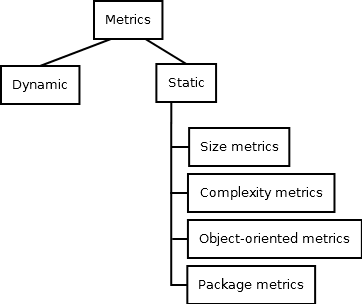
\includegraphics[scale=0.7]{img/Diagram1.png} 
	\caption{Static and dynamic metrics}		
	\label{fig:metrics1}
\end{figure}

The metrics could be also divided into three categories: product metrics, process metrics and project metrics. Product metrics describe the characteristics of the product such as size, complexity, design features, performance, and quality level. Process metrics are used to improve maintenance and development of software, for example: the effectiveness of defecting removal during development, the pattern of testing defect arrival, and the response time of the fix process. Project metrics describe the project characteristics and execution, for example: the number of software developers, the life cycle of the software, cost, productivity, and schedule. Metrics could belong to multiple categories. For example, the quality metrics are both process metrics and project metrics \cite{metrics}. 

\begin{figure}[h!]
	\centering
	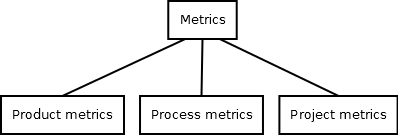
\includegraphics[scale=0.5]{img/Diagram2.png} 
	\caption{Metrics division}		
	\label{fig:metrics2}
\end{figure}


%%%%%%%%%%%%%%%%%%%%%%%%%%%%%%%%%%%%%%%%%%%%%%%%%%%%%%%%%%%%
\section{Software Quality Model}
Experienced software developers are able to create a high quality software, however it is possible only when from the beginning all requirements and expectations are clearly defined. Having the overall view it is possible to design the system that has understandable and minimal complex structure. 

However, the situation often changes after first release. It could happen so, because the client expectations were different or have changed, or new functionality need to be added, or the requirements have been clarified. In that case, the system loses its quality and get out of control. Testing, maintaining and extending software become a nightmare for developing team. 

In order to keep development projects on the right track, and decrease the consequences of situations described above, several general software quality models gained the acceptance within the software engineering community. First people that described quality models are McCall and Boehm \cite{rigorous}. Figure \ref{fig:boehmjpg} presents Boehm`s view, while Figure \ref{fig:mccalljpg} illustrates how McCall viewed quality.

\begin{figure}[h!]
	\centering
	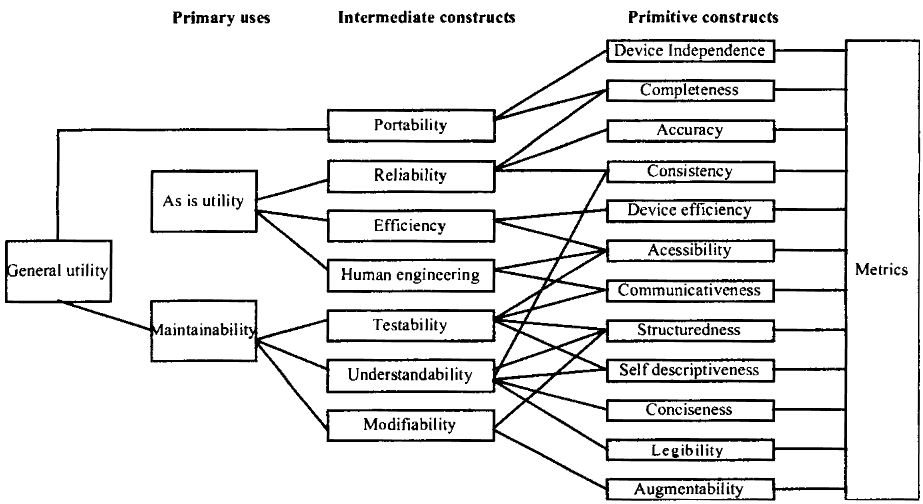
\includegraphics[scale=0.5]{img/boehm-model.jpg}
	\caption{Boehm software quality model (image source:~\cite{rigorous})}		
	\label{fig:boehmjpg}
\end{figure}


\begin{figure}[h!]
	\centering
	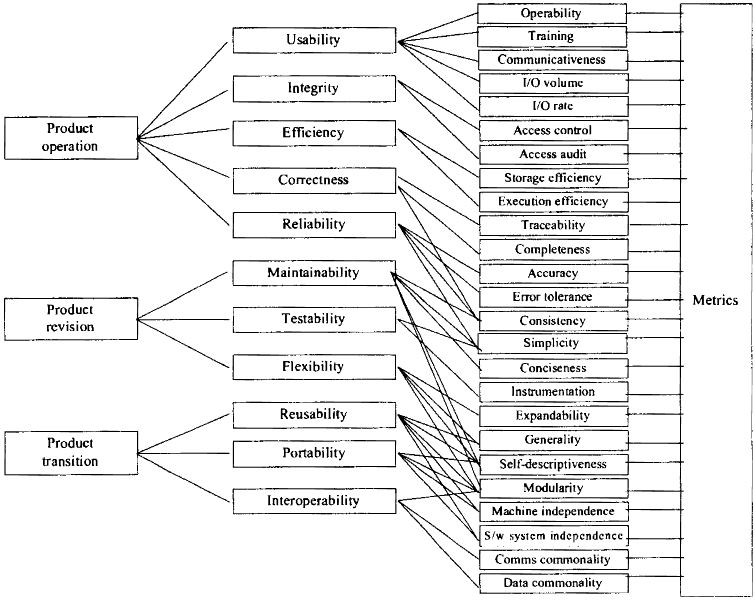
\includegraphics[scale=0.5]{img/mcCall-model.jpg} 
	\caption{McCall software quality model (image source:~\cite{rigorous})}		
	\label{fig:mccalljpg}
\end{figure}

These models focus on the final product (the executable code) and identify the attributes of quality from users point of view. The attributes are called \textit{quality factors}. Because the quality factors names are still too general and no meaningful, they are decomposed into lower-level attributes called \textit{quality criteria}. A further level of decomposition is required when quality criteria are connected to set of low-level, directly measurable attributes called \textit{metrics}. 

\begin{figure}[h!]
	\centering
	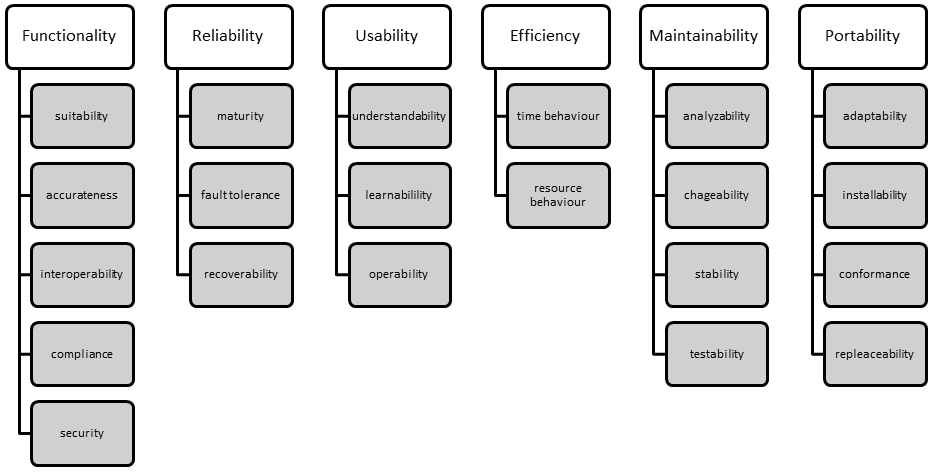
\includegraphics[scale=0.6]{img/diag.png} 
	\caption{The ISO 9126 standard quality model}		
	\label{fig:iso9126}
\end{figure}

From derivation of McCall model, the basic international standard for software quality measurement was defined. The standard is more commonly referenced by its assigned standard number, ISO-9126. It defines software quality as\textit{ ``the totality of features and characteristics of a software product that bear on its ability to satisfy stated or implied needs''} \cite{ISO9126}. The six factors decompose the quality into: 

\begin{itemize}
  \item functionality 
  \item reliability
  \item usability
  \item efficiency
  \item maintainability
  \item portability   
  \end{itemize}
    
\subsection{Functionality}
Functionality is the main purpose of any software. For certain type of software is relatively easy to define its functionality. However, the more functions a software has, the more complicated it becomes. For example, sales order processing systems should be able to record customer information so that it can be used to reference a sales order.

The main point to note is that functionality is expressed as a totality of essential functions that the software product provides. The presence or absence of some functions in a software product can be verified as either existing or not (given function could be or not be found in software product). The other software lcharacteristics present only some degree, because it cannot be simple stated that it characteristic is presented or not. The ISO-9126 quality model does not help measure overall process but only the software component. The relationship between software functionality within an overall business process is outside the scope.

There are five software quality criteria that characterize the usefulness of the software in a given environment (Table~\ref{tab:functionality_factor}):

\begin{table}[h!]
	\centering
\begin{tabular}{|l|l|}
\hline
{\bf quality criteria} & {\bf explanation} \\
\hline
suitability & appropriateness to specification, functions of the software. \\
\hline
accurateness & correctness of the functions \\
\hline
interoperability & ability of software components to interact with other components \\
\hline
compliance & compliant capability of software  \\
\hline
  security & unauthorized access to the software functions \\
\hline
\end{tabular}	
	\caption{\textit{Functionality quality factor}}
	\label{tab:functionality_factor}
\end{table}


\subsection{Reliability}
Reliability is defined as capability of the system to being maintained and its service provision under defined conditions for defined periods of time. From one side of this characteristic is fault tolerance that is the ability of a system to withstand component failure. For example if the connection to the server cannot be established for 30 seconds then system informs the users and follows failure procedures (Table~\ref{tab:reliability_factor}). 

\begin{table}[h!]
	\centering
\begin{tabular}{|l|l|}
\hline
{\bf quality criteria} & {\bf explanation} \\
\hline
  maturity & frequency of failure of the software \\
\hline
fault tolerance & ability of software to withstand (and recover) from failure \\
\hline
recoverability & ability to bring back a failed system to full functionality \\
\hline
\end{tabular}	
	\caption{\textit{Reliability quality factor}}
	\label{tab:reliability_factor}
\end{table}


\subsection{Usability}
Usability is defined with regard to functionality and refers to the ease of use for a given function. For example, the most common functions are exposed on the ribbon to be easily access. The ability to learn how to use a system is also a major sub characteristic of usability. The Table~\ref{tab:usability_factor} depicts the quality criteria of usability:

\begin{table}[h!]
	\centering
\begin{tabular}{|l|l|}
\hline
{\bf quality criteria} & {\bf explanation} \\
\hline
understandability & \parbox[t]{12cm}{easiness of system understanding relating to human-computer\\ interaction methods\\} \\
\hline
learnability & learning effort for target users \\
\hline
operability & ability of using software in given environment \\
\hline
\end{tabular}	
	\caption{\textit{Usability quality factor}}
	\label{tab:usability_factor}
\end{table}


\subsection{Efficiency}
Efficiency  is concerned with the system resources used to provide required functionality. For example: amount of disk space, memory, network etc. provides a good indication of this characteristic (Table~\ref{tab:efficiency_factor}).

\begin{table}[h!]
	\centering
\begin{tabular}{|l|l|}
\hline
{\bf quality criteria} & {\bf explanation} \\
\hline
time behaviour & response time for user input \\
\hline
resource behavior & refers to hardware resources: cpu, disk, network usage \\
\hline
\end{tabular}	
	\caption{\textit{Efficiency quality factor}}
	\label{tab:efficiency_factor}
\end{table} 


\subsection{Maintainability}
Maintainability is characterized as ability to identify and fix a fault within a software component. It is impacted by code readability or complexity as well as modularization. Quality criteria that help with identification of the cause of a fault and then fixing the fault is the concern of maintainability.  One of the sub characteristics of maintainability is also the ability to verify (or testing) a system (Table~\ref{tab:maintainability_factor}). 

\begin{table}[h!]
	\centering
\begin{tabular}{|l|l|}
\hline
{\bf quality criteria} & {\bf explanation} \\
\hline
analyzability & ability to indentify cause of failure \\
\hline
changeability & amount of effort need to change a system \\
\hline
 stability & impact of system after change  \\
\hline
testability & effort needed to verify a system change \\
\hline
\end{tabular}	
	\caption{\textit{Maintainability quality factor}}
	\label{tab:maintainability_factor}
\end{table}



\subsection{Portability}
Portability is characteristic referring to how well the software could adopt to changes in its environment or with its requirements (Table~\ref{tab:portability_factor}). 

\begin{table}[h!]
	\centering
\begin{tabular}{|l|l|}
\hline
{\bf quality criteria} & {\bf explanation} \\
\hline
adaptability & ability of change after adding extension \\
\hline
installability & effort needed to install software \\
\hline
conformance &  ability to adjust after changing external component (i.e. database) \\
\hline
replaceability & ability to replace any component with other  \\
\hline
\end{tabular}	
	\caption{\textit{Portability quality factor}}
	\label{tab:portability_factor}
\end{table} 

\subsection{Software quality model summary}
Basing on the measurement aspects of quality model, several separate definition could be stated. This definitions reflect the software usage or realities of system testing and, what is more, could be treated as software metrics. 

The simplest example is portability term expressed as:
\begin{equation}
Portability\quad =\quad 1-\frac { ET }{ ER } 
\end{equation} 
where ET is a measure of the resources needed to move the system to the target environment and ER is a measure of the resource needed to create the system for a resident environment. 

The interpretation of measurements based on quality factors described in ISO-9126, McCall or Boehm models is rather subjective. The objective measurements are more preferable, however the subjective opinion is better than no feedback.  

The comprehensive picture of software quality is presented by six factors. Normally, the measurement should follow  by some defined standards, however, in that case, the methods of measurement and interpretation are defined by end users and developers~\cite{rigorous}.

%%%%%%%%%%%%%%%%%%%%%%%%%%%%%%%%%%%%%%%%%%%%%%%%%%%%%%%%%%%%%%%%%%%%%%%%%%%%%%%%
\section{Size metrics}

Each product of software development could be treated as physical entity and it could be described in terms of its size. It is straightforward and relatively simple to measure. 

\subsection{Lines of Code}
\ac{LoC} is the simplest metric used to measure the size of the program by counting the lines of code. It is the oldest and most widely used size metric. It is very simple concept that have its basics in Assembler programming where every physical line of code was presenting  one instruction. Nowadays, in high level programming languages, the concept have broken down, because of differences between physical lines and instructions statements. As a result, the several variations have been created in order to improve basic \ac{LoC}:

\begin{itemize}
\item \ac{LoC} that counts only executable lines,
\item \ac{LoC} that counts executable lines plus data definitions,
\item \ac{LoC} that counts executable lines, data definitions and comments,
\item \ac{LoC} that counts executable lines, data definitions, comments, and job control language,
\item \ac{LoC} that counts lines as physical lines on a input screen,
\item \ac{LoC} that counts lines as terminated by logical delimiters~\cite{metrics}.
\end{itemize}

There are two major types of  \ac{LoC} measurement: physical \ac{SLoC} and \ac{LLoC}. The specific definition of them are varied. \ac{SLoC} is a line counter in the text of the program's source code including comment and blank lines. \ac{LLoC} attempts to measure number of executable statements, but specific for given computer language. \ac{SLoC} is sensitive to irrelevant code formatting and depends of the programmer code style convention. 

\ac{LLoC} is better metrics, because it estimates the complexity of a single file, class or procedure. Since \ac{LLoC} is not affected by comments, blanks or line continuation, it is a supportive way to measure the amount of the actual programming work. A program with a higher \ac{LLoC} does more than a program with a lower \ac{LLoC}. By adding features, the \ac{LLoC} increases. By deleting features, the \ac{LLoC} should decrease. 

The main advantages of \ac{LoC} is automatic counting,  however used only for a specific language, because it cannot be used for other languages due to the syntax and structural differences among languages.  \ac{LoC} metric is also very intuitive because the effect of it could be visualized. However, there are many disadvantages that underlines the simplicity of this metrics. Using \ac{LoC} it is not possible to measure the productivity of a project. The final number of lines in program is dependent to the experience of the developer,  for instance, the same functionality could be rewritten by experienced developers using smaller number of lines of code. What is more, any form of \ac{LoC} does not take into consideration code redundancy.  There is no standard definition of what a line of code is. It is not clearly defined whether data declarations are included or  does the comments count or  what happens if a statement extends over several lines. 

In relation to \ac{LoC}, several additional terms has been also defined: 
\begin{itemize}
\item KLOC can be used to measure thousands of \ac{LoC}.
\item KDLOC: 1,000 delivered lines of code
\item KSLOC: 1,000 source lines of code
\item MLOC: 1,000,000 lines of code
\item GLOC: 1,000,000,000 lines of code
\end{itemize}

Summing up, the lines of code metric is one of the oldest and most common forms of software measurement, however is ineffective at comparing the same piece of code of implemented functionality in different languages. It cannot measure the productivity of programmer and code quality~\cite{metrics}.

%%%%%%%%%%%%%%%%%%%%%%%%%%%%%%%%%%%%%%%%%%%%%%%%%%%%%%%%
\subsection{Code coverage}
\label{sec:codecoverage}

Edsger Dijkstra said: \textit{``Testing never proves the absence of faults, it only shows their presence''}.
The code coverage analysis is a measurement used in software testing to describe the degree to which the source code of a program has been tested. There are number of criteria (metrics) that determines how well the tests exercise the code.

The main purpose of code coverage analysis is not only finding the areas of a program not exercised by set of tests, but also creating additional test to increase the coverage or just to identify redundant test cases that does not increase coverage. Using code coverage analysis, it is also important to establish the minimum and maximum percentage of coverage in order to determine when to stop analysing the coverage. 

Code coverage analysis is kind of structural testing technique (other names: glass box testing and white box testing). Structural testing compares behaviour of test program against the direct  intention of the source code. This is a contrast to functional testing (other name: black-box testing) that compares behaviour of test program against a requirements specification. Structural testing examines how the program works, taking into account possible faults in the structure and logic. Functional testing examines what the program accomplishes, without regarding to how it works internally.

There are variety of coverage metrics. The paragraphs below contain a description of some fundamental metrics, their strengths, weaknesses and issues. 

\paragraph{Statement coverage metrics} reports every executable statement that is encountered.  Note that a statement does not necessarily correspond to a line of code. Control-flow statements, such as \texttt{if, for} and \texttt{switch} are covered if the expression controlling the flow is covered as well as all the contained statements. Implicit statements, such as an omitted return, are not subject to statement coverage. 

Advantage of statement coverage is verification of what the written code is expected to do and not to do. It also measures the quality of written code, checks the flow of different paths in the program and it also ensures, if those path are tested or not.

Disadvantage of statement coverage is fact that it cannot test the false conditions. It does not report if the loop reaches its termination condition and it does not understand the logical operators.

Statement coverage is also called \textit{statement execution, line, block, basic block} or \textit{segment coverage}.

It could be quite difficult to achieve 100\% statement coverage, because it might be sections of code designed to deal with error conditions, or rarely occurring events. There may also be code that should never be executed.

The statement coverage can be calculated as shown below:
\begin{equation}
Statement\quad coverage\quad =\quad \frac { number\quad of\quad statement\quad exercised }{ total\quad number\quad of\quad statements } \cdot 100\%
\end{equation}


%%%%%%%%%%%%%%%%%%%%%%%%%%%%%%%%%%%%%%%%%%%%%%%%%%%%%%%%
\paragraph{Decision coverage metrics} also known as \textit{branch coverage} or \textit{all-edges coverage}. It covers both the true and false conditions.  A branch is considered as the outcome of a decision and it  simply measures which decision outcomes have been tested. This metrics takes a more in-depth view of the source code than simple statement coverage.

A decision is taken in if-statement, a loop control statement  or a switch statement and the result of these statements could be either TRUE or FALSE.

The advantages of decision coverage is possibility to validate all the branches in the code, because all of them are reached. It is done in order to ensure that no branches lead to any not normal program`s operation. This metric eliminates also problems that occur with statement coverage testing. 

The decision coverage can be calculated as given below:
\begin{equation}
Decision\quad coverage\quad =\quad \frac { Number\quad of\quad decision\quad outcomes\quad exercised }{ Total\quad number\quad of\quad decision\quad outcomes } \cdot 100\%
\end{equation}

The main goal of decision coverage is to ensure if a program could jump and it jumps to all possible destinations. The most simple example is a complete if statement:
\begin{lstlisting}[caption=Decision coverage metric passes,label=lst:decisionpass]
if (x) {
	print "a";
} else {
	print "b";
}
\end{lstlisting}
This coverage is only achieved here only if \texttt{x} is true on one occasion and false on another.

%%%%%%%%%%%%%%%%%%%%%%%%%%%%%%%%%%%%%%%%%%%%%%%%%%%%%%%%
\paragraph{Condition coverage metric} reports the true or false outcome of each condition separately. It measures the conditions independently of each other. It is similar to decision coverage but has better sensitivity to the control flow. During boolean expression evaluation it is need to ensure that all the terms in the expression are exercised. For example:

\begin{lstlisting}[caption=Simple conditional coverage, label=lst:conditional]
if (x || y) {
	//...
} 
\end{lstlisting}

In order to achieve the full condition coverage of this expression, the values of x and y are set to each of the four combinations of values they can take:

\begin{verbatim} 
x=true; y=true;
x=true; y=false;
x=false; y=true;
x=false; y=false;
\end{verbatim} 

The condition coverage gets complicated, and difficult to achieve, as the expression gets complicated. For this reason there are a number of different ways of reporting condition coverage which try to ensure that the most important combinations are covered without worrying about less important combinations.

\begin{lstlisting}[caption=Complex conditional coverage, label=lst:conditional2]
if (a || b) && c {
	//...
}
\end{lstlisting}

The condition will be satisfied by the following set of tests:
\begin{verbatim} 
a=true, b=true, c=true
a=false, b=false, c=false
\end{verbatim} 

However, it does not satisfy the condition coverage, because it need to test rest of possibilities:
\begin{verbatim}
a=false, b=false, c=true
a=true, b=false, c=true
a=false, b=true, c=true
a=false, b=true, c=false
\end{verbatim}

Condition coverage is also known as \textit{expression, condition-decision} and \textit{multiple decision coverage}.
%%%%%%%%%%%%%%%%%%%%%%%%%%%%%%%%%%%%%%%%%%%%%%%%%%%%%
\paragraph{Path coverage metrics} reports if every possible path in given function has been followed. This path is a unique sequence of branches from the function entry to the exit. It tests all possible combinations of logical conditions. 

The purpose of path coverage metrics is to ensure that all paths through the program are taken. In sizeable program there will be an enormous number of paths through the program could be executed, so in practice the paths could be limited to those within a single function whether the function is not too big, or i.e. has simply two consecutive branches.

The main advantage of path coverage metrics is accuracy. However, from the other side, the number of path increase exponentially to the number of branches and it is impossible to exercise all of time in small unit of time.  

%%%%%%%%%%%%%%%%%%%%%%%%%%%%%%%%%%%%%%%%%%%%%%%%%%%%%
\subsubsection{Other coverage metrics} 
There are also many other variation of coverage metrics like\textbf{ function coverage metric} that reports when function or procedure is invoked. The \textbf{call coverage metric} reports every function call. The \textbf{ loop coverage metric} informs whether each loop body has been executed zero times, exactly once or more than once. For supporting multi threading the \textbf{race coverage} reports whether multiple threads execute the same code at the same time. It supports with detecting failures with synchronization of resource access. The \textbf{relational operator coverage} reports if the boundary situations occur with operators: \textit{\textless, \textless=, \textgreater, \textgreater=,==}. 

%%%%%%%%%%%%%%%%%%%%%%%%%%%%%%%%%%%%%%%%%%%%%%%%%%%%%
\subsubsection{Coverage metrics summary}
The result of using statement coverage, decision coverage, or condition coverage should attain 80\%-90\% coverage or more before releasing. It does assure quality and the effort sacrificed to reach this goal, might be supportive in finding more bugs. The good project avoids setting a goal lower than 80\%.

The coverage analysis help eliminate gaps in a test suite. It does not only provide accurate measurements in order to be useful, but also encourage software developers to analyse those results to the minimum detail and support them in decision how code could be improved ~(\cite{coverage1},~\cite{coverage2}).

%%%%%%%%%%%%%%%%%%%%%%%%%%%%%%%%%%%%%%%%%%%%%%%%%%%%%
\subsection{Code size metrics summary}
Internal attribute of product like size is important and measuring it directly allows to predict the complexity. Number of characters, lines of code or code coverage is taken into account as a determinant for these kind of metrics.  

Basing on \ac{LoC} it is possible to calculate derivative metrics like productivity quality or \textit{``documentation--size''} metrics: 

\begin{equation}
productivity=\frac { KLOC }{ man-month } 
\end{equation}
 
 \begin{equation}
quality\quad =\quad \frac { bugs }{ KLOC } 
\end{equation}

\begin{equation}
documentation\quad size\quad =\quad \frac{documentation\quad pages }{KLOC} 
\end{equation}

It is worthy to mention that these kind of metrics are only supportive way of monitoring improvement of software development and it is not allowed to evaluate the code developers basing on results of these metrics. 

%%%%%%%%%%%%%%%%%%%%%%%%%%%%%%%%%%%%%%%%%%%%%%%%%%%%%
\section{Complexity metrics}

Computational complexity has also impact on the software, so if the complex algorithms are used in software, there is a need to control the overall efficiency of program execution. The complexity metrics provide the information how complex the implemented methods in code are. The sections below describes the basic and commonly used complexity metrics. 
 
\subsection{McCabe's cyclomatic complexity}
\label{sec:cyclomatic}
McCabe has based its metrics on analysis of some measurement concepts in graph theory. He has  transferred these concepts into domain of software measurement. The terms connected to graph theory have been explained in Chapter~\ref{section:graph_theory} in section: \textit{Graph theory}. The term \textit{cyclomatic number} is explained below (definition from:~\cite{alain}).

\begin{quote}
\textit{The \ac{CC} number \textbf{v(G)} of a strongly connected directed graph is equal to the
maximum number of linearly independent cycles.}
\end{quote}\vspace{-1cm}

\begin{equation}
v(G) = e - v + p
\end{equation}

where:
\begin{itemize}\addtolength{\itemsep}{-0.5\baselineskip}\vspace{-7mm}
\item \textit{G} represents the graph,
\item \textit{e} represents the edges of the graph,
\item \textit{v} represents the vertices,
\item \textit{p} represents separate components.
\end{itemize}

The entity being measured is therefore a \textit{``strongly connected directed graph''}. In software, the program is modelled with usage of \textit{control flow graph} that represents abstract structure. In this abstract representation of a program or a procedure, each vertex in the graph represents a basic block, directed edges are used to depicts the jumps in the flow control. There are also two additional designed blocks: entry block through which control flow enters the flow graph and the exit block through which all control flow leaves.  

The Figure~\ref{fig:cyclomatic_complexity} represents the exemplary flow control graph.

\begin{figure}[h!]
	\centering
	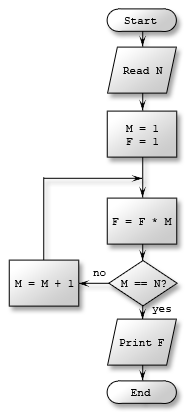
\includegraphics[scale=0.5]{img/cyclomatic_complexity.png} 
	\caption{Example of \ac{CC}: 8 vertices (nodes), 8 edges; $CC = 8 - 8 + 1 = 1$; image source:~\url{http://upload.wikimedia.org/wikipedia/commons/1/16/Flowchart_example.png}.}		
	\label{fig:cyclomatic_complexity}
\end{figure}

In the case of software, the control flow graph is transformed into a strongly connected graph, so graph cyclomatic number could be formulated as:

\begin{equation}
v(G) = e - v + p + (1\quad virtual \quad edge)
\end{equation} 

Furthermore, the individual modules are also taken into consideration, instead of the whole software entity. According to McCabe, the number of connected component $p$ is equal to 1, so the final McCabe equation is formulated as:

\begin{equation}
v(G) = e - v + 2
\end{equation}

where $e$ is a number of edges and $v$ is a number of vertices. It is also another formula that gives the simple \ac{CC} dependent to the number of vertices:

\begin{equation}
v(G) = d + 1
\end{equation}
where $d$ is number of decision vertices points in code where the binary decision are made. This formula allows to quick determination of \ac{CC} value by counting how many in code, the keywords \texttt{if, while, for, switch, case, do, catch} are used. 

The low value of \ac{CC} determines that given function is easy to understand. The greatest value is, the more complicated code is. What is more, the more complex code is, the more faults could appear~\cite{alain}.
%%%%%%%%%%%%%%%%%%%%%%%%%%%%%%%%%%%%%%%%%%%%%%%%%%%%%

\subsection{Halstead complexity}
The Halstead's metrics were proposed by Maurice Halstead. The main assumption is to determine a quantitative measure of the complexity directly from the operators and operands in the component. Metrics measure program component's complexity directly from source code, because the implementation or expression of the algorithm should reflect the execution independently of a specific platform. The main goal is to identify measurable software properties and its relations.

Halstead metrics are based on interpretation of the source code as a sequence of tokens and classifying them to be either operator or operand.   

An operand is the part of a computer instruction which specifies what data is to be manipulated or operated on. The operator, in programming, has the same definition as in mathematics. It is a character that represents the specific action performed on the variables (addition, subtraction, multiplication, comparison, incrementation,...). 

The \textbf{program length (N)} is the sum of the total number of operators and operands in the program:
\begin{equation}
N={ N }_{ 1 }+{ N }_{ 2 }
\end{equation}

The \textbf{vocabulary size (n)} is the sum of the number of unique operators and operands:
\begin{equation}
n={ n }_{ 1 }+{ n }_{ 2 }
\end{equation}

The \textbf{program volume (V)} is the contents of program information. It is measured in mathematical bits and is calculated as the program length times the 2-base logarithm of the vocabulary size (n) :
\begin{equation}
V=N\cdot \log _{ 2 }{ n } 
\end{equation}

Halstead's volume (V) describes the size of the implementation of an algorithm. The computation of V is based on the number of operations performed and operands handled in the algorithm. The program volume (V) is less sensitive to code layout than the lines-of-code measures\footnote{The definition of Halstead's metrics described above are not a part of complexity metrics, but size metrics, however these metrics are used as a base for metrics describes below which are categorized as complexity metrics. Using Halstead's size metrics is meaningless without Halstead's complexity metrics, so it is a reason why they have been introduced and explained in the same section.}. 

The \textbf{difficulty level or error proneness (D)} of the program is proportional to the number of unique operators in the program. D is also proportional to the ratio between the total number of operands and the number of unique operands. 
\begin{equation}
D=\frac { { n }_{ 1 } }{ 2 } \cdot \frac { { N }_{ 2 } }{ { n }_{ 2 } } 
\end{equation}
        
The \textbf{program level (L)} is the inverse of the error proneness of the program. I.e. a low level program is more prone to errors than a high level program.
\begin{equation}
L=\frac { 1 }{ D } 
\end{equation}
        
The \textbf{effort to implement (E)} is proportional to the volume and to the difficulty level of the program. It is also known as program understanding or elementary mental discrimination.
\begin{equation}
E=V\cdot D=\frac { V }{ L } =\frac { { n }_{ 1 }{ N }_{ 2 }{ Nlog_{ 2 }{ n } } }{ 2{ n }_{ 2 } } 
\end{equation}

The \textbf{time to implement (T)} is proportional to the effort. Empirical experiments could be used for calibrating this quantity. Halstead has found that dividing the effort by Stroud Number $S$ gives an approximation for the time in seconds.
\begin{equation}
T=\frac { E }{ S } =\frac { { n }_{ 1 }{ N }_{ 2 }{ Nlog_{ 2 }{ n } } }{ 2{ n }_{ 2 }S } 
\end{equation}

In 1967, psychologist John M. Stroud suggested that the human mind is capable of making a limited
number of mental discrimination per second (Stroud Number), in the range of 5 to 20. The $S$ value for software scientists is set to 18, thus: 

\begin{equation}
T=\frac { E }{ 18 } 
\end{equation}

\subsection{Complexity metrics summary}
The advantage of Halstead metrics is fact that it does not require in-depth and control flow analysis of program. They are able to predicts an effort and rate the error and estimate the time, so they are useful in scheduling projects. As a drawbacks of Halstead metrics, it could be noticed that it depends on usage of operator and operands in completed code and it has no use in predicting complexity of program at design level.

Calculating the ~\ac{CC} value from the McCabe metric is rather easy. This metric determines also which application elements should be redesigned and reimplemented. However, on the other side, the number of edges in control flow does not give the full answers, because it does not distinguish nested and not nested loops from easy \texttt{case} instruction. It also does not take into account complicated conditions in decision vertices~\cite{complexity1}.


%%%%%%%%%%%%%%%%%%%%%%%%%%%%%%%%%%%%%%%%%%%%%%%%%%%%%%
\section{Object-oriented metrics}
Object-oriented metrics are a response to the object-oriented programming paradigm that is not reflected in the methods of structure programming measurements.   

\subsection{Chidamber \& Kemerer metrics}
\ac{CK metrics} is the set of metrics proposed by S.R. Chidamber and C.F Kemerer in 1994. They have explored features characteristic for object-oriented design: class complexity, inheritance, coupling and cohesion between classes.   
\paragraph{\ac{WMC}} is a weighted sum of method from given class where single weight is represented as McCabe cyclomatic complexity. \ac{WMC} is a sum of all coefficients of \ac{CC} in given class and is expressed in formula:

\begin{equation}
WMC=\sum _{ i=0 }^{ TM }{ { CC }_{ i } } 
\end{equation}
where $TM$ - number of method in class, $CC_{i}$ - cyclomatic complexity of \textit{i}-method. Recommended \ac{WMC} value should be equal to 20. The value has been determined by NASA scientists. They based its assumptions on experience in object-oriented projects~\cite{nasa}.

\paragraph{\ac{RFC}} is the number of methods that can be invoked in response to a message in a class. In other words, all methods from given class and all methods which are invoked directly by these methods are counted. The greater \ac{RFC} value is, the greater functionality and complexity is. It causes that the cost of testing and maintaining the system also increases. Such value means also more responsible for a class. The desirable value determined by NASA is 40~\cite{nasa}.

\paragraph{\ac{DIT}} is defined as a maximal number of super classes that given class inherits.  The inheritance tree depth are characteristic for complex systems. It involves a wide range of related classes and methods and means higher cost of system maintenance. On the other hand, inheritance increases the reuse of code, which reduces the number of duplicate code~\cite{nasa}.

\paragraph{\ac{NOC}} is defined as sum of all direct class descendants. Large \ac{NOC} values indicate improper usage of inheritance mechanism and might result in difficulties in class testing and maintaining~\cite{nasa}.  

\paragraph{\ac{CBO}} is defined as a number of classes that are coupled with given class using other mechanism than inheritance. The low level of class coupling indicates that class are independent and there are clear boundaries between them. It increases the abstraction of project, because it is easier to modify the code. The high level of \ac{CBO} makes class more sensitive to changes and difficult to maintain, therefore relationship between classes should be kept at as low level as possible. It reduces the complexity of the system and promotes better encapsulation~\cite{nasa}. 

\paragraph{\ac{LCOM}} is type of metric that measures lack of cohesion of methods in class. There are several version of calculating \ac{LCOM}.

\subparagraph*{LCOM1} is a difference between number of pairs of methods that refers to different attributes over the pair of methods referring to at least one common attribute. 

Let the class have $n$ methods $m_{1}, m_{2}, \cdots, m_{n}$ where $I_{j}$ is a set of attributes used by $m_{j}$ method. It could be defined: $P=\left\{ \left( { I }_{ i },{ I }_{ j } \right) :{ I }_{ i }\cap { I }_{ j }=0 \right\}$ and $Q=\left\{ \left( { I }_{ i },{ I }_{ j } \right) :{ I }_{ i }\cap { I }_{ j }\neq 0 \right\}$, so: 

\begin{equation}
LCOM1=P-Q\quad if\quad P>Q\quad or\quad LCOM1=0\quad otherwise
\end{equation}

High value indicates that responsibility for given class is too high and class should be divided into smaller, because it is more difficult to test and maintain given class. During next years the \ac{LCOM} metric has been several times redefined. 

\subparagraph*{LCOM2} is represented as per cent of methods that do not have access to individual class attributes. If number of method or attributes is equal to zero, then LCOM2 is also not defined and is equal to zero. 

\begin{equation}
LCOM2=1-\frac { \sum _{ i=1 }^{ TM }{ { Ma }_{ i } }  }{ TM\times TA } 
\end{equation}
where $TM$ is number of method in class, $TA$ is number of attributes in class and $Ma_{i}$ is number of methods that refers to $a_{i}$ attributes. The results of this metric are in interval between 0 and 1. The lowest value, the better is. 

\subparagraph*{LCOM3} is a relative number of methods that do not refer to individual class attributes.

\begin{equation}
LCOM3=\frac { TM-\frac { \sum _{ i=1 }^{ TM }{ { Ma }_{ i } }  }{ TA }  }{ TM-1 } 
\end{equation}

where $TM$ is number of method in class, $TA$ is number of attributes in class and $Ma_{i}$ is number of methods that refers to $a_{i}$ attributes. The results are in interval between 0 and 2. If number of attributes is equal to 0 or number of methods is 1 then metric is not defined. The values greater than 1 indicates lack of cohesion and probability of dividing class on smaller ones in future. 

\subparagraph*{LCOM4} is number of disjoint sets of local methods. Neither of these two sets disjonts. Each two methods within the same set have access to at least one common attributes. Value of this metric is between 0 and $N$ where $N$ is a natural number. Optimal value is equal to 1. For greater values it is need to divide class on smaller classes. 

%%%%%%%%%%%%%%%%%%%%%%%%%%%%%%%%%%%%%%%%%%%%%%%%%%%%%
\subsection{Metrics for Object-Oriented Design (MOOD)}
\ac{MOOD} were created by Fernando Brito e Abreu in 1995. They are expressed in per cents and used to overall system evaluation. It determines the degree of the usage of mechanisms characteristic for object-oriented programming. The \ac{MOOD} set is programming language independent. 

\ac{MOOD} measures the following object-oriented characteristics:

\begin{itemize}\addtolength{\itemsep}{-0.5\baselineskip}\vspace{-7mm}
\item  polymorphism:~\ac{PF}
\item encapsulation (hermatization):~\ac{AHF}~and~\ac{MHF}
\item inheritance:~\ac{AIF}~and~\ac{MIF}
\item messaging:~\ac{CF}
\end{itemize}\vspace{-10mm}

\paragraph{Polymorphism Factor} defines the degree of classes overridden in subclasses.
\begin{equation}
PF=\frac { \sum _{ i=1 }^{ TC }{ { m }_{ o }({ c }_{ i }) }  }{ \sum _{ i=1 }^{ TC }{ \left[ { m }_{ n }({ c }_{ i })\times dc({ c }_{ i }) \right]  }  } 
\end{equation}
where $TC$ - the number of all classes, $c_{i}$ - the following classes, $m_{n}(c_{i})$ - new methods, $m_{0}(c_{i})$ - inherited methods, $dc(c_{i})$ - descendants of $c_{i}$ class. 

The nominator represents the number of possible different polymorphic situation
and the denominator represents the maximum number of possible distinct polymorphic
situation for class $c_{i}$. Polymorphism enables to link, by its own invocation, many instance of classes, so system becomes more complex and flexible. The typical \ac{PF} value is between 4\% and 18\%. The greater value is, the more complicated inheritance hierarchy is. This situation causes increase the cost of maintenance and testing (\cite{moodbook}, \cite{nasa}). 

\paragraph{Attribute Hiding Factor} defines the degree of attributes encapsulation in class.
\begin{equation}
AHF=\frac { \sum _{ i=1 }^{ TC }{ { a }_{ h }({ c }_{ i }) }  }{ \sum _{ i=1 }^{ TC }{ { a }_{ d }({ c }_{ i }) }  }
\end{equation}
where $TC$ - the number of all classes, $c_{i}$ - the following classes, $a_{h}$ - non-public attributes, $a_{d}$ - all defined attributes in $c_{i}$ class. The~\ac{AHF} value should be close to 100\% because it is one of basic assumption of encapsulation that attributes are only accessible using methods (\cite{moodbook}, \cite{nasa}).

\paragraph{Method Hiding Factor} defines the degree of method encapsulation in class.
\begin{equation}
MHF=\frac { \sum _{ i=1 }^{ TC }{ { m }_{ h }({ c }_{ i }) }  }{ \sum _{ i=1 }^{ TC }{ { m }_{ d }({ c }_{ i }) }  } 
\end{equation}
where $TC$ - the number of all classes, $c_{i}$ - the following classes, $m_{h}$ - non-public methods, $m_{d}$ - all defined methods in $c_{i}$ class. The desirable value of~\ac{MHF} should be between 10\% and 25\%, because some of methods are not available at all (\cite{moodbook}, \cite{nasa}).


\paragraph{Attribute Inheritance Factor} defines the degree of attributes inheritance usage. It is a ratio of inherited and all available attributes. 
\begin{equation}
AIF=\frac { \sum _{ i=1 }^{ TC }{ { a }_{ i }({ c }_{ i }) }  }{ \sum _{ i=1 }^{ TC }{ { a }_{ a }({ c }_{ a }) }  } 
\end{equation}
where $TC$ - number of all classes, $a_{a}(c_{i}) = a_{d}(c_{i}) + a{i}(c{i})$ - public attributes in $c_{i}$ class, $a_{i}(c_{i})$ - inherited and not overridden attributes in $c_{i}$ class, $a_{d}(c_{i}) = a_{n}(c_{i}) + a_{o}(c_{i})$ - attributes defined in $c_{i}$ class, where $a_{n}(c_{i})$ - new attributes, $a_{o}(c_{i})$  - inherited and overridden attributes. The typical value of \ac{AIF} is between 50\% and 60\% (\cite{moodbook}, \cite{nasa}).  


\paragraph{Method Inheritance Factor} defines the degree of methods inheritance usage. It is a ratio of inherited and all available methods. 
\begin{equation}
MIF=\frac { \sum _{ i=1 }^{ TC }{ { m }_{ i }({ c }_{ i }) }  }{ \sum _{ i=1 }^{ TC }{ { m }_{ a }({ c }_{ a }) }  } 
\end{equation}
where $TC$ - number of all classes, $m_{a}(c_{i}) = m_{d}(c_{i}) + m_{i}(c_{i})$ - public methods in $c_{i}$ class, $m_{i}(c_{i})$ - inherited and not overridden methods in $c_{i}$ class, $m_{d}(c_{i}) = m_{n}(c_{i}) + m_{o}(c_{i})$ - methods defined in $c_{i}$ class, where $m_{n}(c_{i})$ - new methods, $m_{o}(c_{i})$  - inherited and overridden methods. The typical \ac{MIF} value is between 65\% and 80\%. The values below indicates weak usage of inheritance, otherwise, the values greater than 80\% complicates the inheritance and code re-usage (\cite{moodbook}, \cite{nasa}).   


\paragraph{Coupling Factor} defines the degree of coupling between classes using different methods than inheritance. It is a ratio of number of couplings between classes with use of aggregation, composition, association and maximal number of couplings that could be used in system.  
\begin{equation}
CF=\frac { \sum _{ i=1 }^{ TC }{ \left[ \sum _{ j=1 }^{ TC }{ is\_ client\left( { c }_{ i },{ c }_{ j } \right)  }  \right]  }  }{ { TC }^{ 2 }-TC+2\times \sum _{ i=1 }^{ TC }{ dc({ c }_{ i }) }  } 
\end{equation}	
where $TC$ - number of all classes, $dc(c_{i})$ - descendants of $c_{i}$ class, ${TC}^{2}-TC$ - maximal number of possible couplings in $TC$ class system, $2\times \sum _{ i=1 }^{ TC }{ dc({ c }_{ i }) }$ - maximal number of coupling using inheritance in system,  $is\_ client\left( { c }_{ i },{ c }_{ j } \right) = 1\quad if\quad { c }_{ c }\Rightarrow { c }_{ s }\wedge { c }_{ c }\neq { c }_{ s }\wedge \neg \left( { c }_{ c }{ \rightarrow c }_{ s } \right) $ otherwise $is\_ client\left( { c }_{ i },{ c }_{ j } \right) =0$. The ${ c }_{ c }\Rightarrow { c }_{ s }$ expression means that class $c_{c}$ has at least one reference to class $c_{s}$. The ${ c }_{ c }{ \rightarrow c }_{ s }$ expression means that  class $c_{c}$ inherits class $c_{s}$. The \ac{CF} value is between 5\% and 15\%. The high value means that system is not flexible and is difficult to maintain and test, because one change in the system requires modifications in another parts of system. Small value means that classes are too complex, not cohered and it realizes too much functionality inside (\cite{moodbook}, \cite{nasa}).  
	%%%%%%%%%%%%%%%%%%%%%%%%%%%%%%%%%%%%%%%%%%%%%%%%%%%%%%
\section{Package metrics}

Package metrics are used to measure software at the package level. They are used to evaluate the correctness of coupling. The most popular set of package metrics were introduced by Robert C. Martin.

\subsection{Martin metrics}
Martin metrics are set of five metrics designed by Robert Cecil Martin in 1994. His metrics \textit{``can be used to measure the quality of an object-oriented design in terms of the interdependence between the subsystems of that design, because designs which are highly interdependent tend to be rigid, unreusable and hard to maintain''}~\cite{martin}.

\paragraph{\ac{Ce}} is also known as \textit{Outgoing Dependencies}. This metric measures all the types from the source of the measured package referring to the types not in the measured package~\cite{martin}. A large \ac{Ce} indicates that a package is unfocussed and unstable, because it depends on the stability of all the types to which it is coupled. The recommended value of \ac{Ce} is upper limit of 20. The \ac{Ce} could be reduced by extracting some parts of classes and decomposing into smaller and more specialized classes. The typical example of large valued efferent coupling are GUI elements which covers all logical operation within a software.

\paragraph{\ac{Ca}} determines how many classes and interfaces from other packages depend on classes in analysed package. It is also known as \textit{Incoming Dependencies}. The number of packages that depend on the analysed package indicates the package level of responsibility. If the package is relatively abstract then a large number of incoming dependencies is acceptable. Otherwise if not, the package is more concrete. The acceptable values are much larger than in the case of \ac{Ce}. The allowed value for \ac{Ca} is about 500. It is caused by difficulty of the control of the packages which depend on the analysed package. An example of \ac{Ca} high value is controller from MVC pattern~\cite{martin}.

\paragraph{\ac{I}} is measured by calculating the effort necessary  to change a package without impacting other packages within the application. Instability is also called \textit{Stable Dependencies Principle}. The number of incoming and outgoing dependencies is an indicator that determines the stability and instability of a package. Instability can be calculated by comparing the incoming and outgoing package dependencies:

\begin{equation}
I\quad =\quad \frac { Ce }{ Ca+Ce } 
\end{equation}

The returned value is in the range between 0.0 and 1.0 where 0.0 indicates a maximally stable package and 1.0 indicates a maximally unstable package. However, it is impossible to clearly state about stability of package, so it have been assumed that package is stable within range: 0.0 to 0.3 and unstable from 0.7 to 1.0.

Summing up, the package containing multiple outgoing but few incoming dependencies is less stable because of the consequences after introducing changes. On the other hand, package containing more incoming dependencies are more stable because it is more difficult to change~\cite{martin}.


\paragraph{\ac{A}} calculate a relationship between number of  abstract classes and interfaces within package and total number of concrete (non-abstract) classes in the same package. The abstractness is calculated using the formula:

\begin{equation}
A=\frac {N_{a}}{N_{c}} 
\end{equation}

where $N_{a}$ is a number of abstract classes and interfaces in a package and $N_{c}$ is a number of concrete classes and interfaces in the package. The abstractness value of zero ($A=0$) indicates that package contains complete concrete classes. The abstractness value of one ($A=1$) indicates that package is completely abstract. 

Having abstractness value in range between 0 and 0.5 determines that package is opened to changes of implementation. However it could be stated so, whether this value will be compared to instability of package. If package is highly unstable, it would be hard to change because of stability and such package cannot be extended because it is not abstract.

If the abstractness value is closed to 1, the package is unstable and it should consist of concrete classes. It is need to limit dependences to unstable types. Using abstract classes as unstable types will cause increased of dependences to them, because, in case of abstract classes, it is need to create class that will inherit from abstract class~\cite{martin}.


\paragraph{\ac{D}} points that abstractness and stability of packages are closely connected. This metrics is expressed using the formula:

\begin{equation}
D = A + I - 1
\end{equation}

The ideal value is $D=0$, what means that the more abstract a package is, the more stable it should be because it should have many clients that depend on its abstractions.The desirable value should as low as possible~\cite{martin}. Any package that is not closed to zero is considered as unbalanced and should be reimplemented in order to be more reusable and less sensitive to changes.

\section{Other software metrics}
\label{sec:other-metrics}
There are also many other software metrics that are commonly used to preventing the faults in software. They increase the quality of code and have been implemented in plugins in Eclipse IDE described in Chapter~\ref{roz:metrics-tools}. The alphabetic list presents short description of each of them:  

\textbf{\ac{CLOC}} counts all lines that contain regular comments and Javadoc comments.

\textbf{\ac{COM}} calculates number of comment lines. 

\textbf{\ac{CYC}} estimates how many cycles in which a package is involved.

\textbf{\ac{DC}} determines a density value of how commented the code is and is expressed in formula: $DC = \frac{CLOC}{LOC}$.

\textbf{\ac{DIP}}  calculates the ratio of dependencies that have abstract classes or interfaces as a target.

\textbf{\ac{DCYC}} counts every mutual dependency between packages.

\textbf{\ac{EP}}  calculates the ratio of classes that are used outside of a package.

\textbf{\ac{EXEC}} counts the number of executable statements.	

\textbf{\ac{LC}} indicates density of comments with respect to textual size of program $LC=\frac {LOC}{COM}$.

\textbf{\ac{LSP}} is the number of direct subpackages of a package.

\textbf{\ac{NOA}}  calculates the number of fields declared in class or interface.

\textbf{\ac{NCLOC}} (aka NCSL and ELOC) counts all the lines that do not contain comments or blank lines.

\textbf{\ac{NOF}}  calculates the number of fields declared in method.

\textbf{\ac{NOM}} indicates number of modules (packages).

\textbf{\ac{NOTa}} counts the number of abstract classes and interfaces.

\textbf{\ac{NOTc}} counts the number of concrete classes.	

\textbf{\ac{NOTe}} counts the number of classes and interfaces exported outside a package.

\textbf{\ac{NP}} counts the number of parameters for a method or a constructor.

\textbf{\ac{NOT}} counts the number of classes and interfaces.

\textbf{\ac{MC}} indicates density of comments with respect to logical complexity of program $LC=\frac { CC }{ COM } $.

\section{Summary}
[dodac zawartosc ;)]
